\documentclass{scrartcl}
\usepackage{my}
\usepackage{subcaption}
\usepackage{biblatex}
\addbibresource{satyakisen-conformalprediction.bib}

\title{Conformal Prediction}
\author{Satyaki Sen \\ 
\footnotesize{Email: {rvusmail@gmail.com}} \\
Mentor: Sima Noorani \\
\footnotesize{University of Pennsylvania, Email: {nooranis@engineering.upenn.edu}}}
\begin{document}
\maketitle


\section{Introduction}
Machine learning models are widely used to make predictions and answer questions for many tasks.
However, it is important to be confident in the reliability of such models when using them.
 \emph{Conformal Prediction}, or CP, is a method 
for producing \emph{prediction sets} from the model: sets that are guaranteed to contain the true value
with some user-chosen probability. One of the main advantages of an approach based on CP is that it assumes
little about how the model works, and does not make any strong assumptions about the distribution of the data.

In this document, we survey some of the main ideas of conformal prediction. Section~\ref{sec:cp} is an overview
of the conformal prediction mechanism in general. In sections \ref{sec:classification} and \ref{sec:regression}, we apply these techniques
to classification and regression tasks, with experiments on MNIST and the Communities and Crime dataset. 
Finally, Section~\ref{sec:text} discusses the challenges of using CP on text generation models, and we test one such method
on the TriviaQA dataset.
\section{What is Conformal Prediction?}
\label{sec:cp}

Suppose that we have a model takes objects $x$ from some set $X$
and produces outputs $y \in Y$; these may be answers to questions or predictions for regression. 
Conformal Prediction, a technique introduced by Vovk and collaborators in \cite{vovkbook},
is a wrapper around the model that takes in an input $x$ and produces a prediction set $\Gamma^{\alpha}(x)$.
The main property is that these prediction sets $S \subseteq Y$ from CP are guaranteed to contain
the true answer with probability at least $1 - \alpha$ (here $\alpha$ is some chosen miscoverage threshold).
Here, we will only deal with split conformal prediction, and will not use the ``full'' version of conformal prediction.
The main procedure, which is explained further in \cite{introcp}, is essentially the following steps:

\begin{itemize}
    \item Assign a \emph{non-conformity score} $s(x, y)$ to each pair $(x, y) \in X \times Y$. Intuitively, 
    this measures how strange it would be for
    $y$ to be the true answer for $x$. 
    A better score function provides prediction sets that are more useful, but $1 - \alpha$
    coverage holds no matter what choice of score function $s$ we make.

    \item Over some calibration data $\mathcal{D}_{cal}$, which contains objects $x \in X$ along with the true
    values $y \in Y$, compute the scores $s(x_i, y_i)$ for $(x_i, y_i) \in \mathcal{D}_{cal}$. Then, compute the $1 - \alpha$
    quantile of these scores, which we denote $\hat{q}$. That is, $\hat{q}$ is the value such that only a fraction $\alpha$ of the scores
    are higher than $\hat{q}$. In practice,
    it is often better to compute the $\lceil (n + 1)(1 - \alpha) \rceil/n$ quantile instead of the $1 - \alpha$ quantile,
    where $n = |\mathcal{D}_{cal}|$.

    \item Now, when faced with a new object $x' \in X$, we include a value $y \in Y$ in the prediction set, denoted
    $\Gamma^{\alpha}(x')$, if and only if $s(x', y) \le \hat{q}$.

\end{itemize}

This conformal algorithm works under the assumption that the data we face in practice is \emph{exchangeable}
with the calibration data. For instance, the special case of i.i.d data satisfies this assumption. 
This \emph{split conformal prediction} approach is nice for many reasons:
we assume little about the distribution of the data
that is encountered, and the approach does not care about any specifics of the model itself. 
Because coverage is always guaranteed, the main factor that
tells us how useful the prediction sets are is their size; naturally, smaller sets for the same coverage are more useful.

\begin{proof}[Proof of the conformal coverage guarantee.]
Sort our $n$ calibration scores as $s_1 < s_2 < \dots < s_n$ (here assuming they are distinct),
so that $\hat{q} = s_{\lceil (n + 1)(1 - \alpha) \rceil}$ represents the $\lceil (n + 1)(1 - \alpha) \rceil/n$ quantile of the scores.
Now when we see a new example $x$, we will include $y$, the true label, in the prediction set as long as $s(x, y) \le \hat{q}$.
By exchangeability, when we add $s(x, y)$ to the scores,
it is equally likely to fall at any of the $n + 1$ positions in the ordering of $s_1 < s_2 < \dots < s_n$ together with $s(x, y)$.
Then the chance that its position is at or below $\lceil (n + 1)(1 - \alpha) \rceil$ is
$\lceil (n + 1)(1 - \alpha) \rceil/(n + 1) \ge 1 - \alpha$, which is exactly the coverage guarantee we wanted.
\end{proof}

\section{Classification}
\label{sec:classification}
How do we actually compute the key ingredients of the above process,
the non-conformity scores $s(x, y)$, in a classification setting? A natural choice,
if we have the probabilities assigned by the model
to each class in $Y$, is to define the score by $s(x, y) = 1 - p(y)$. Assuming that the probabilities $p(y)$ are
reasonably well associated with how well class $y$ represents object $x$, this satisfies the desired property:
classes that the model is confident represent $x$ have lower scores,
and classes that the model is less confident about have higher scores.

\begin{figure}[h]
    \centering
        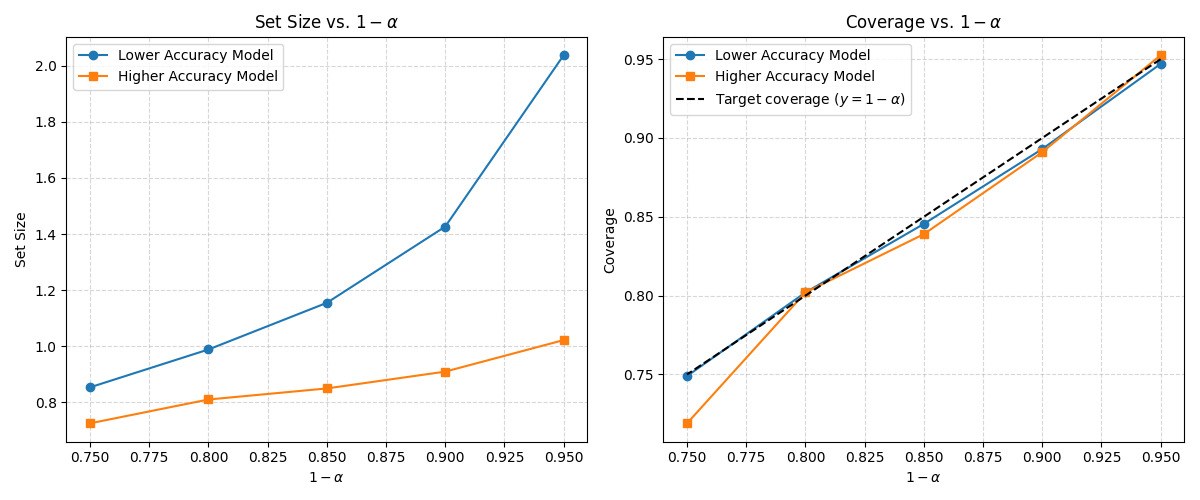
\includegraphics[width=\textwidth]{graphs/conformal_simple_comparison.png}
        \caption{The two models are both MNIST classifiers, with 90\% and 95\% accuracy, respectively.
        We plot the average set size and empirical coverage for both models.}
    \label{fig:simpleCP-comparison}
\end{figure}

Figure~\ref{fig:simpleCP-comparison} demonstrates two characteristics of CP. With a more accurate model, the set sizes can be smaller,
because there is less uncertainty as to what the true label is. Additionally, the conformal algorithm can produce
size $0$ sets, as evidenced by the average set sizes taking values $< 1$. This can happen especially if we request a $1 - \alpha$
lower than the model's base accuracy, since we do not need to add anything to guarantee coverage. For example, if we request $90\%$
coverage on a $95\%$ accuracy model, we can afford to make some set sizes $0$. \medskip

One alternative to the simple score function we used above is known as \emph{APS}, for adaptive prediction sets.
Ideally, with APS, the set sizes should more accurately reflect how difficult or easy the classification question is,
producing larger sets when the model is unsure. Here, we define scores as
\[ s(x, y) \coloneq \sum_{y' : \, p(y') \ge p(y)} p(y'), \]
that is, the score is the sum of all the softmax probabilities that are at least the probability of $y$.
This obeys our intuitive understanding: if there are many classes with probability higher than $y$, then
the model is less confident that $y$ is the answer, and so $s(x, y)$ is higher.

\begin{figure}[h]
    \centering
        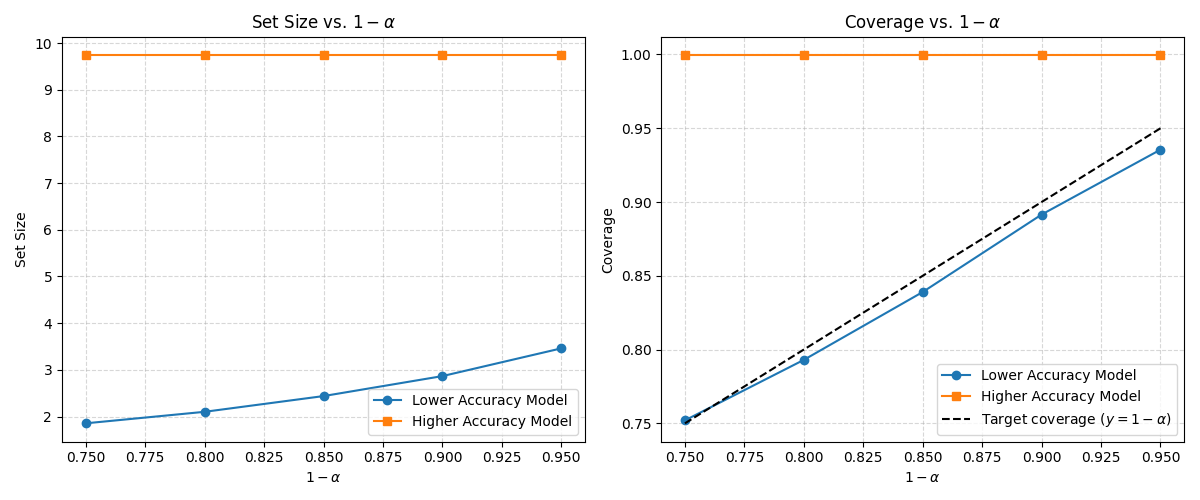
\includegraphics[width=\textwidth]{graphs/conformal_adaptive_comparison.png}
        \caption{Same as Figure~\ref{fig:simpleCP-comparison}, but now using the APS strategy as described above.}
    \label{fig:adaptiveCP-comparison}
\end{figure}

In Figure~\ref{fig:adaptiveCPcomparison}, we see that for the higher accuracy model, the set sizes are nearly always $10$,
the largest possible sets. Despite the APS approach being theoretically better, these results
are not what we expect. The issue here is that with the higher accuracy model,
the model generates one softmax score that is essentially $1$ and the others essentially $0$.
As a result, there are many ties among the scores: the partial-sum-based scores are all essentially $1$,
leading to the unintended behavior of including all $10$ categories in the prediction sets.
The standard way to deal with tied scores is to introduce a random noise component into the scores, 
which we do in Figure~\ref{fig:RandomAPS-comparison}. Here, the score function is randomized with 
\[ s(x, y) = u \cdot p(y) + \sum_{p(y') > p(y)} p(y') , \]
where $u$ is uniformy random in $(0, 1)$.

\begin{figure}[h]
    \centering
        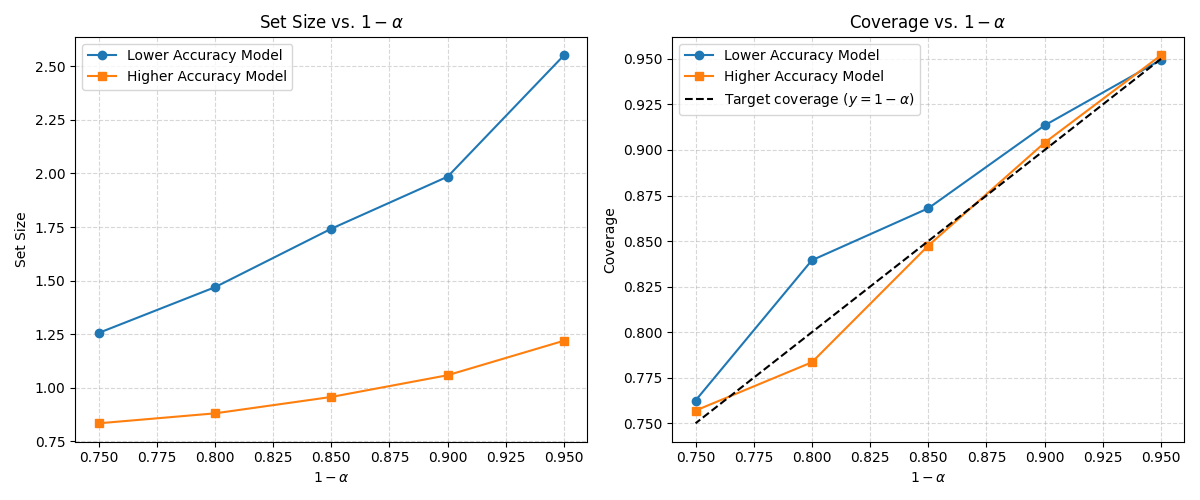
\includegraphics[width=\textwidth]{graphs/conformal_adaptive_random_comparison.png}
        \caption{Same as Figure~\ref{fig:adaptiveCP-comparison}, but now with randomized noise added to the scores as described above.}
    \label{fig:RandomAPS-comparison}
\end{figure}

A variation on the randomized version of APS is the regularized APS algorithm, which aims both to break ties using random noise
and to disincentivize large sets using a \emph{regularization} component. This component discourages the algorithm
from producing prediction sets larger than a certain size.
This algorithm is described in more detail in \cite{rapspaper}. Let $o_x(y)$ be the rank of $y$ in the output probabilities
when they are listed in descending order.
We will use two parameters $\lambda$, $k$ to determine how much we regularize the sets. Then,
    \[ s(x, y) = \max(0, \lambda(o_x(y) - k)) + p(y) \cdot u + \sum_{y' : \, p(y') > p(y)} p(y'), \]
where $u$ is uniformly random in $(0, 1)$. Thus, if for example $k=4$, including anything past the $4$th term
carries an extra penalty of $\lambda$ for each position beyond the $4$th, so we are incentivized to use sets that
do not extend past the $4$th term, hopefully making the set sizes smaller.
The results of this are in Figure~\ref{fig:regularizedCP-comparison}.

\begin{figure}[h]
    \centering
        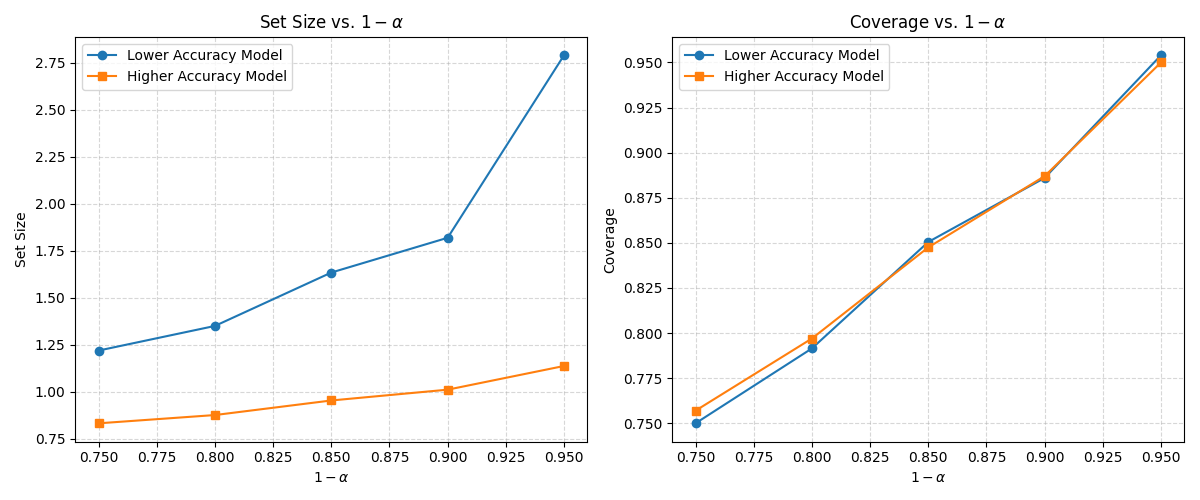
\includegraphics[width=\textwidth]{graphs/conformal_regularized_comparison.png}
        \caption{Using the regularized APS (RAPS) algorithm on MNIST, with $k = 3$, $\lambda = 0.1$.}
    \label{fig:regularizedCP-comparison}
\end{figure}

In our case, for an MNIST classifier, the impact of using regularized APS (RAPS)
versus a simple random-noise-based strategy is not too large.
With only ten labels, everything past the first few labels has probability essentially zero and would not be included anyway.
However, RAPS can make a bigger difference on classification tasks like ImageNet.
When we have large class spaces $Y$ like in ImageNet, a tail of small probabilities forms,
and RAPS stops us from including classes from the tail, thus making the sets smaller and more informative.

\section{Regression}
\label{sec:regression}
Another use case for conformal prediction is when we have a regression model instead of a classification model.
For a simple version of CP for regression, we will start with a \emph{quantile regression} model. Given some data $x$,
it will give us a prediction \emph{interval} $(t_{\alpha/2}, t_{1 - \alpha/2})$ that should contain the correct value $y$
with coverage $1 - \alpha$. However, this coverage is not guaranteed, because a quantile regression model will not be perfectly fitted.
To guarantee $1 - \alpha$ coverage, we can apply conformal prediction.
Define the score of $(x, y)$ to be how far $y$ is from the predicted quantiles, that is,
\[ s(x, y) = \max(t_{\alpha/2} - y, y - t_{1 - \alpha/2} ) .\]
Because of the way we have defined this score function, if $y$ indeed lies within the predicted interval,
the score $s(x, y)$ will be negative, and it will be positive if $y$ is outside the interval. 
To create the prediction sets, we follow the mechanism in Section~\ref{sec:cp}, including $y$ when $s(x , y) \le \hat{q}$.
Thus, the conformalized
interval is widened or shrunk based on $\hat{q}$: it will be $(t_{\alpha/2} - \hat{q}, t_{1 - \alpha/2} + \hat{q})$. The results of using this algorithm, known as \emph{CQR}
(conformalized quantile regression), are shown in Figure~\ref{fig:simpleRegression-comparison}.

\begin{figure}[h!]
    \centering
    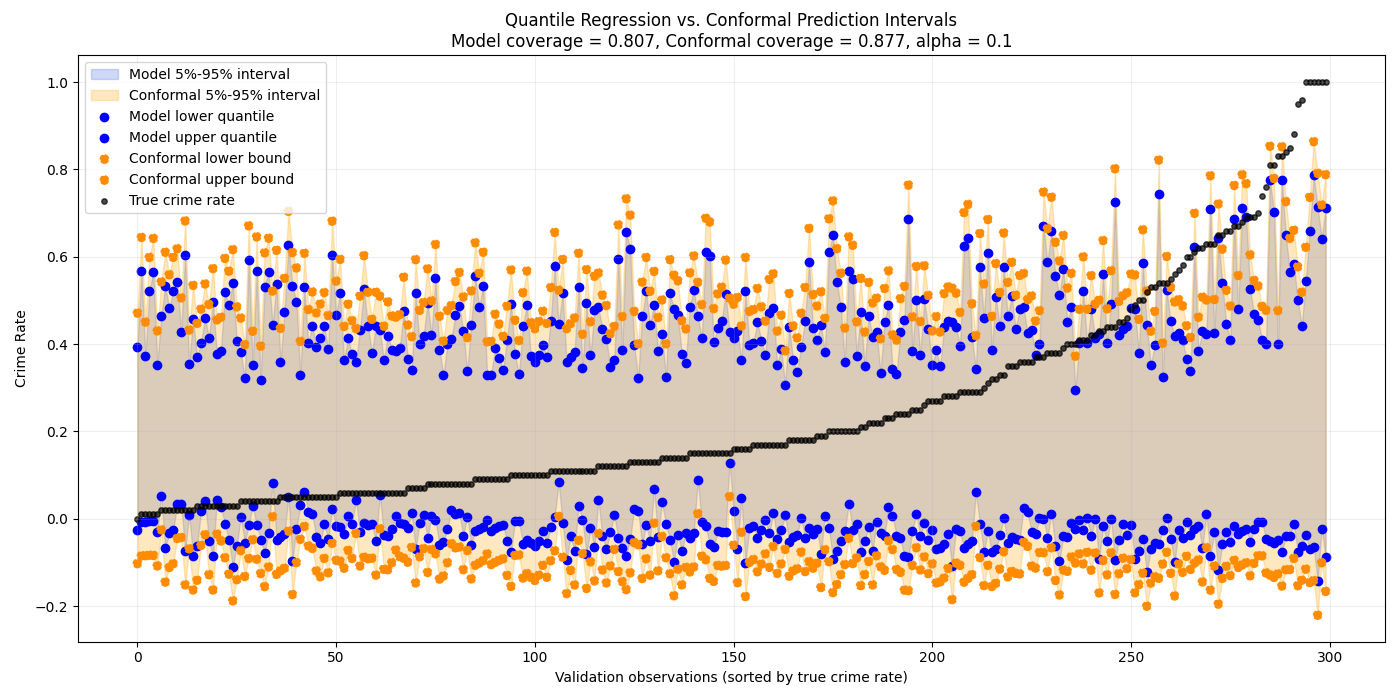
\includegraphics[scale=0.4]{graphs/badNNregressionCQRscatterV2.png}
    \caption{CQR on the \emph{Communities and Crime} dataset, predicting the crime rate in a community from data about that community.
    Here the inputs contain $122$ features about a community, and the desired output is the crime rate of that community.}
    \label{fig:simpleRegression-comparison}
\end{figure}

As an alternative to the CQR algorithm, we can adjust the prediction sets in a more adaptive way,
depending on both $\hat{q}$ and some estimate of the uncertainty of a prediction. In this case,
we begin with a model that estimates $y$ from $x$, producing $\hat{y}$. We then also need
some uncertainty scalar $u(x)$, predicted by a second model or by an additional output of the same model;
this can be an estimate of the residual, the standard deviation, or something else.
The scores are then
\[ s(x, y) = \frac{| \hat{y} - y |}{u(x)} , \]
and the prediction sets are constructed as $(\hat{y} - \hat{q}u(x), \hat{y} + \hat{q}u(x))$.
This method, called \emph{Uncertainty Scalars}, is shown in Figure~\ref{fig:UncertaintyScalars}.
Note that in Figure~\ref{fig:UncertaintyScalars}, we compute the uncertainty scalar as the width of the interval,
$u(x) = |t_{1 - \alpha/2} - t_{\alpha/2}|$, which is a reasonable estimate of uncertainty: if the model is more confident,
the interval will be smaller, and if the model is less confident, the interval will be larger.

\begin{figure}[h]
    \centering
    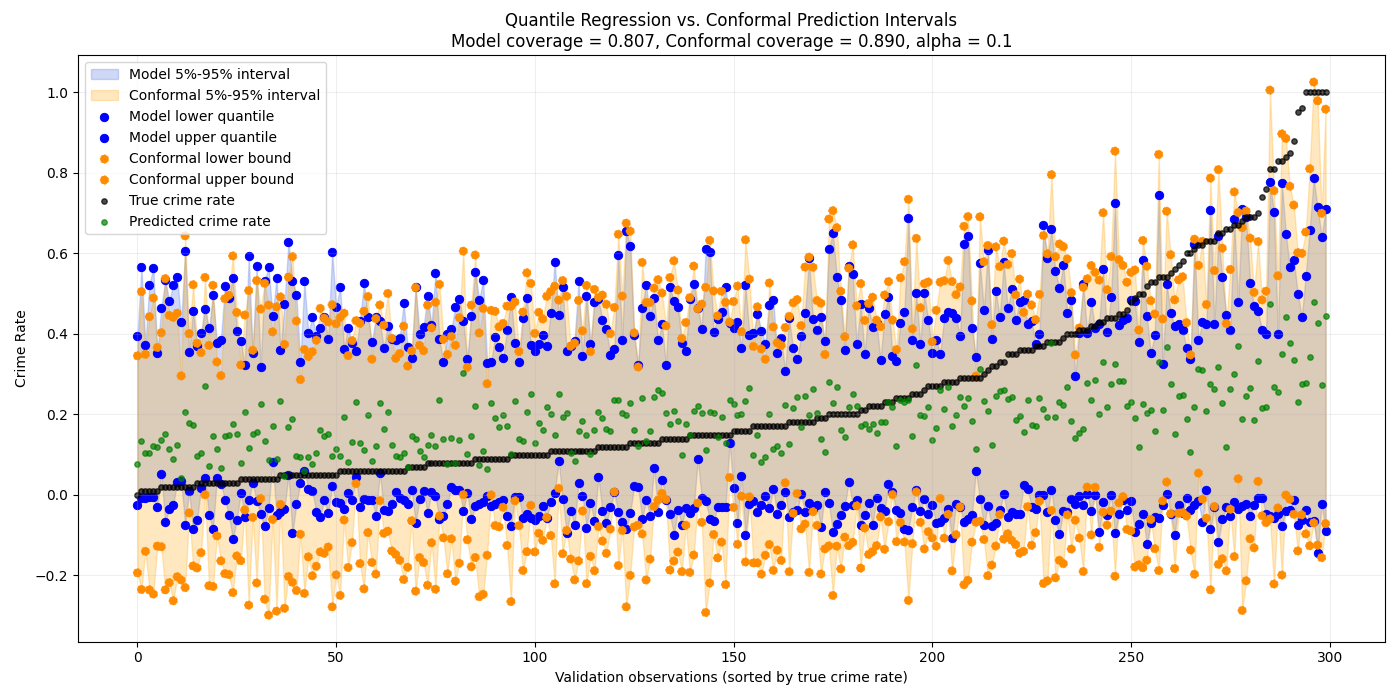
\includegraphics[scale=0.4]{graphs/NNregressionAdaptive_badV2.png}
    \caption{Uncertainty scalars given by $u(x) = |t_{1 - \alpha/2} - t_{\alpha/2}|$, with a model predicting both the true value and the quantiles on Communities and Crime.}
    \label{fig:UncertaintyScalars}
\end{figure}

\section{Text}
\label{sec:text}
Trying to apply conformal prediction techniques to a language model generating answers to questions
poses a more difficult challenge. For one, text outputs are much less structured than in a classification or regression scenario.
For instance, multiple different-looking outputs can really be the same answer, like ``New York City'' and ``NYC''.
Secondly, there is effectively an infinite space of possible outputs.
Most importantly, we (in general) will not have any more information from a query $x$ than what the model outputs, since we are dealing
with black-box models and know nothing about the actual token probabilities.
Given these hurdles, how can we assign scores $s(x, y)$?
It is clear that we will need to sample the model many times in order to get any information. Then the simplest thing
that we can do here is to compute probabilities from these $n$ outputs:
\[ p(y) = \frac{\text{number of times $y$ was output}}{n}, \]
and let $s(x, y) = 1 - p(y)$. Immediately, we run into an issue: many equivalent outputs $y_i$ can be slightly different,
and so are counted as different by this probability even though they are not. Thus, we must perform \emph{semantic clustering} on the results. That is, we group the results $y_1, \dots, y_n$ into clusters $Y_1, \dots, Y_k$ containing
equivalent responses. One way to do this is to simply ask the model itself to judge entailment between two responses;
then $y_i \equiv y_j$ when $y_i$ entails $y_j$ and $y_j$ entails $y_i$. Then we compute the score of each cluster $Y_j$ as
\[ s(x, Y_j) = 1 - p(Y_j) = 1 - \frac{\text{number of outputs in } Y_j}{n} ,\]
and apply conformal prediction in the same way we did in Section~\ref{sec:classification}. That is, we are effectively
treating the model as a classification model whose set of classes is the set of clusters seen in the $n$ model outputs. \medskip

To test these algorithms, we evaluate on a subset of the TriviaQA dataset, which contains one-line trivia questions
and answers, using Qwen3-8B to answer questions as well as to judge entailment. It is worth noting that Qwen3-8B
is not very accurate on this dataset by itself: it only achieves around $50\%$ accuracy on a single response. We run the above algorithm with a range of $\alpha$ values and $15$ queries per question in Figure~\ref{fig:simpleCPQ}. \medskip

However, as seen in Figure~\ref{fig:simpleCPQ}, the coverage plateaus around $0.55$, and so we do not meet the conformal
coverage guarantee. The problem here is that with the $n$ queries we make to the model, it is possible the true $y$
was simply not in any of the clusters produced. If this happens with probability more than $\alpha$, there is nothing we can do to restore coverage.
If the answer is not produced in the $n$ queries, no subset of the clusters will ever contain the answer. 
The proof in Section~\ref{sec:cp} relies on the assumption that all answers are given a score, but all answer may not appear in
the clusters produced.


%%\begin{figure}[h]
 %%       \centering
  %%      \includegraphics[width=0.5\textwidth]{FreqHighMin1malpha_vs_coverage.png}
    %%    \vspace{1cm}
      %%  \includegraphics[width=0.5\textwidth]{FreqHighMin1malpha_vs_setsize.png}
        %%\caption{Coverage and Set Size vs $1 - \alpha$ for the algorithm described above. As we can see in the graph, the coverage plateaus, and we cannot guarantee coverage.}

        %%\label{Coverage-SimpleCPQ}

%%\end{figure}
\begin{figure}[ht]
\centering
\resizebox{\textwidth}{!}{%
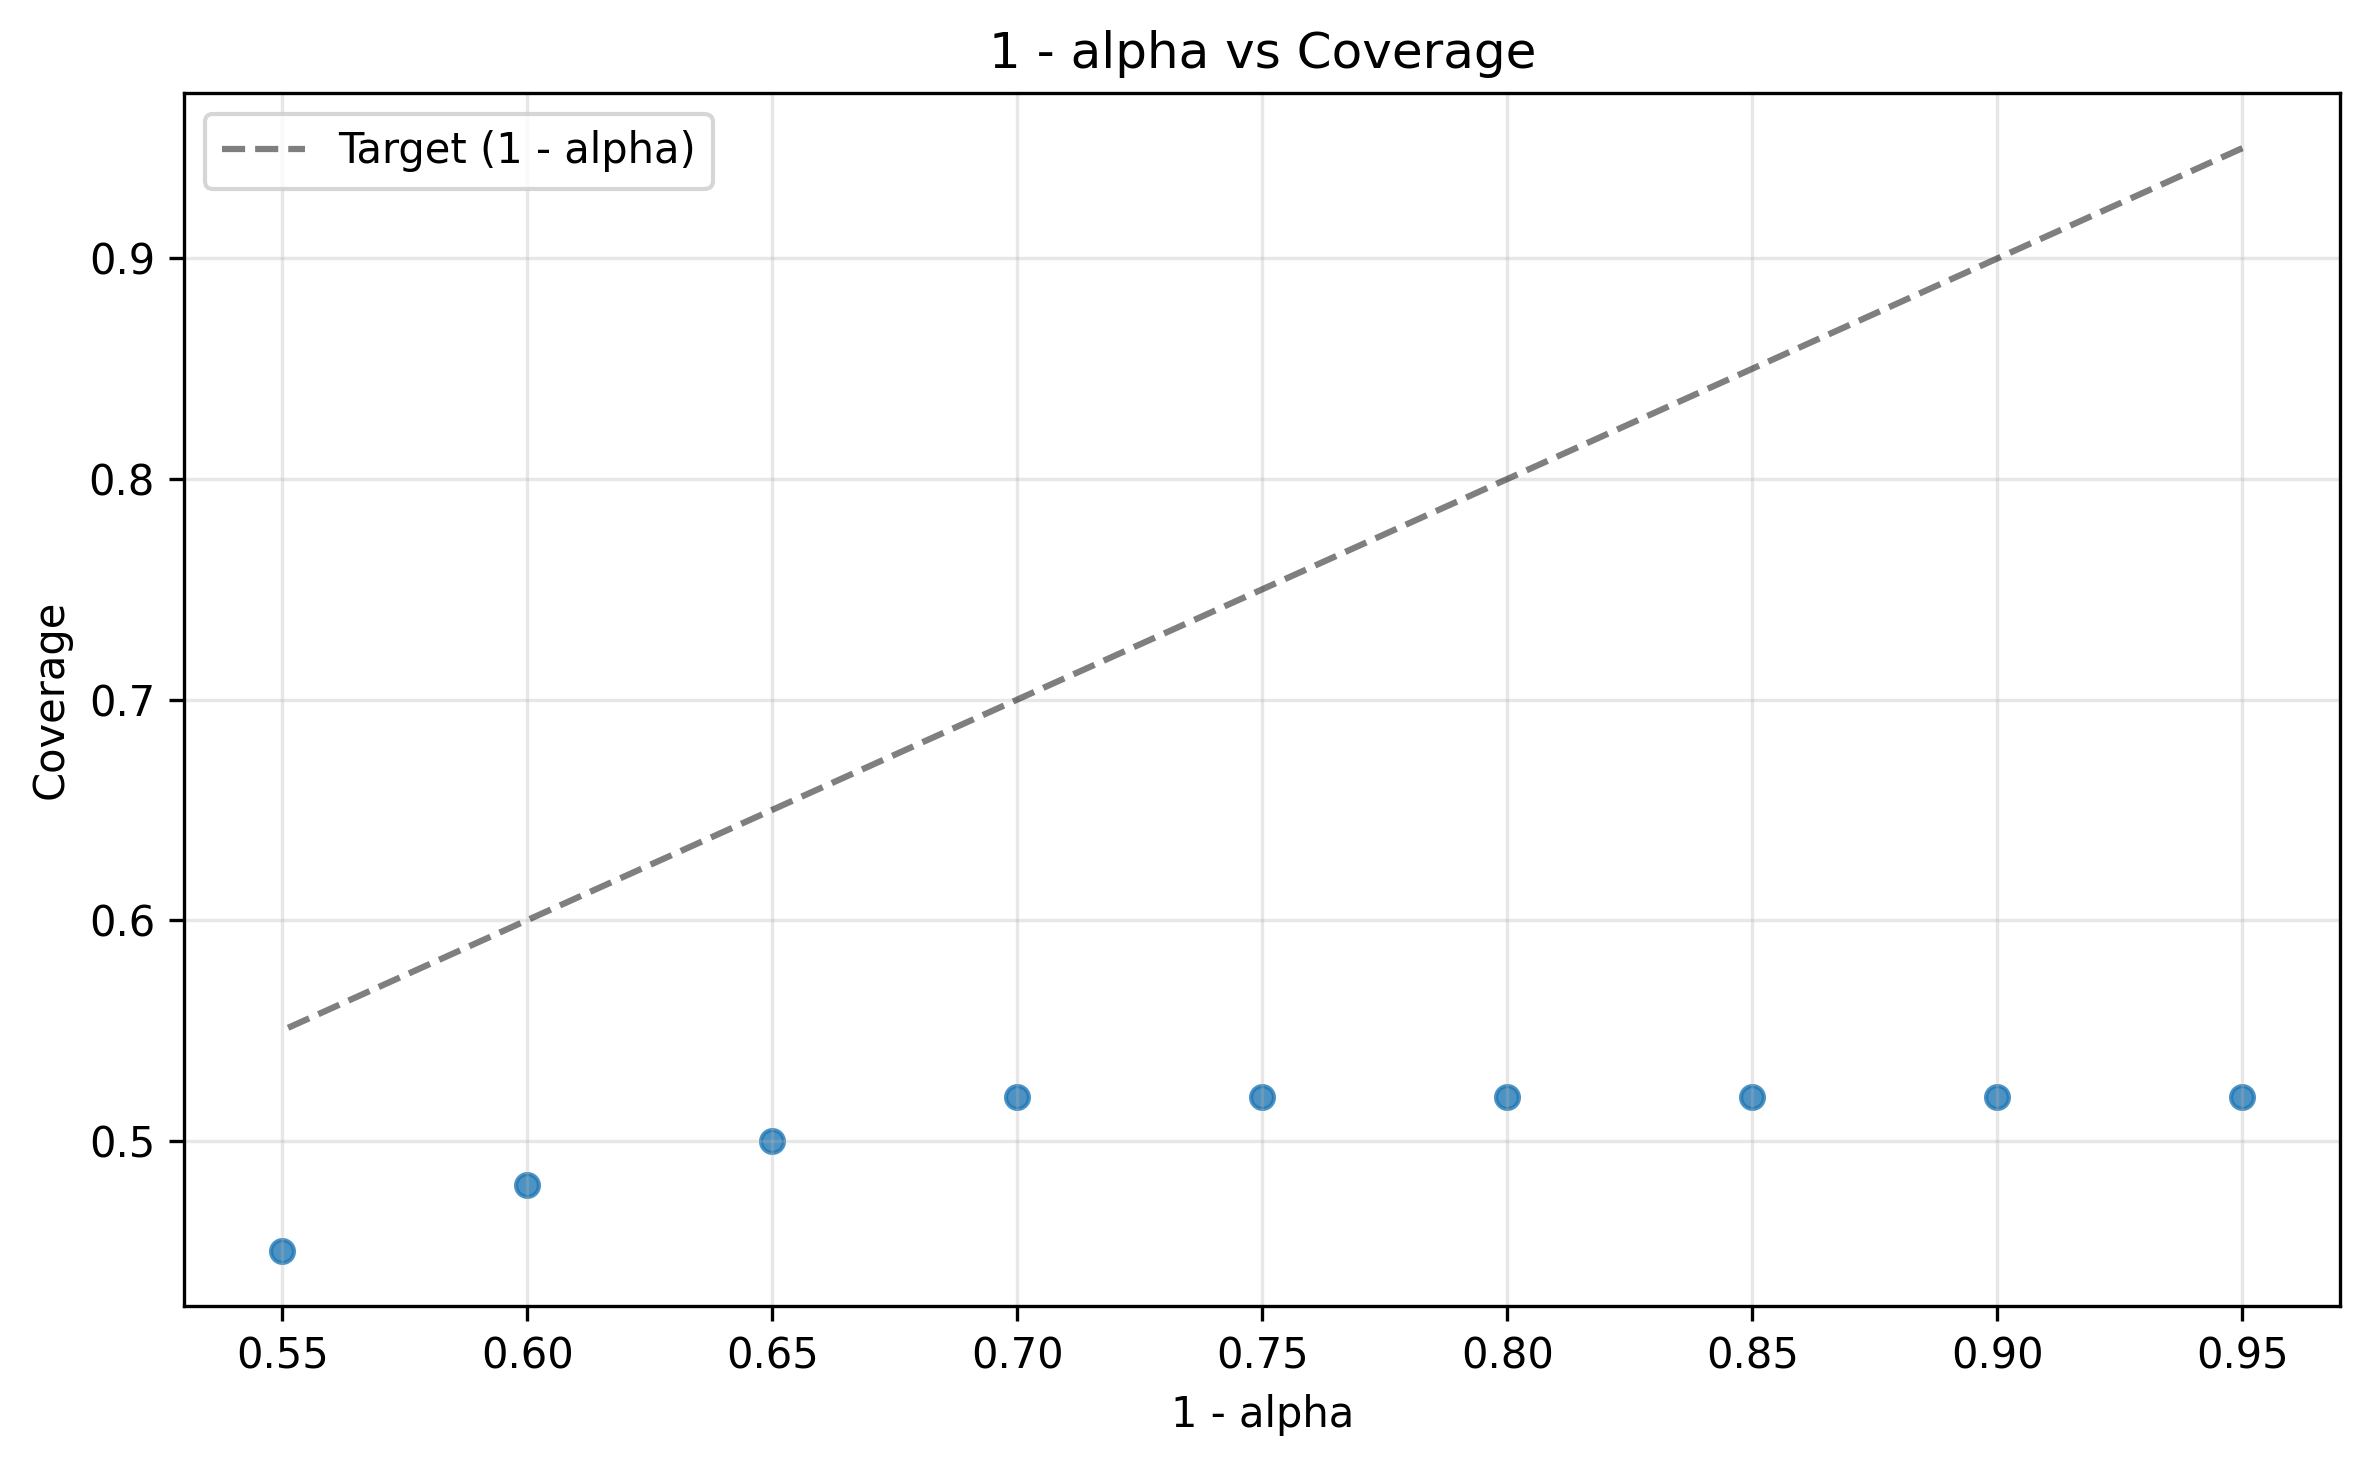
\includegraphics[height=5cm]{cpq/graphs/FreqHighMin1malpha_vs_coverage.png}%
\quad
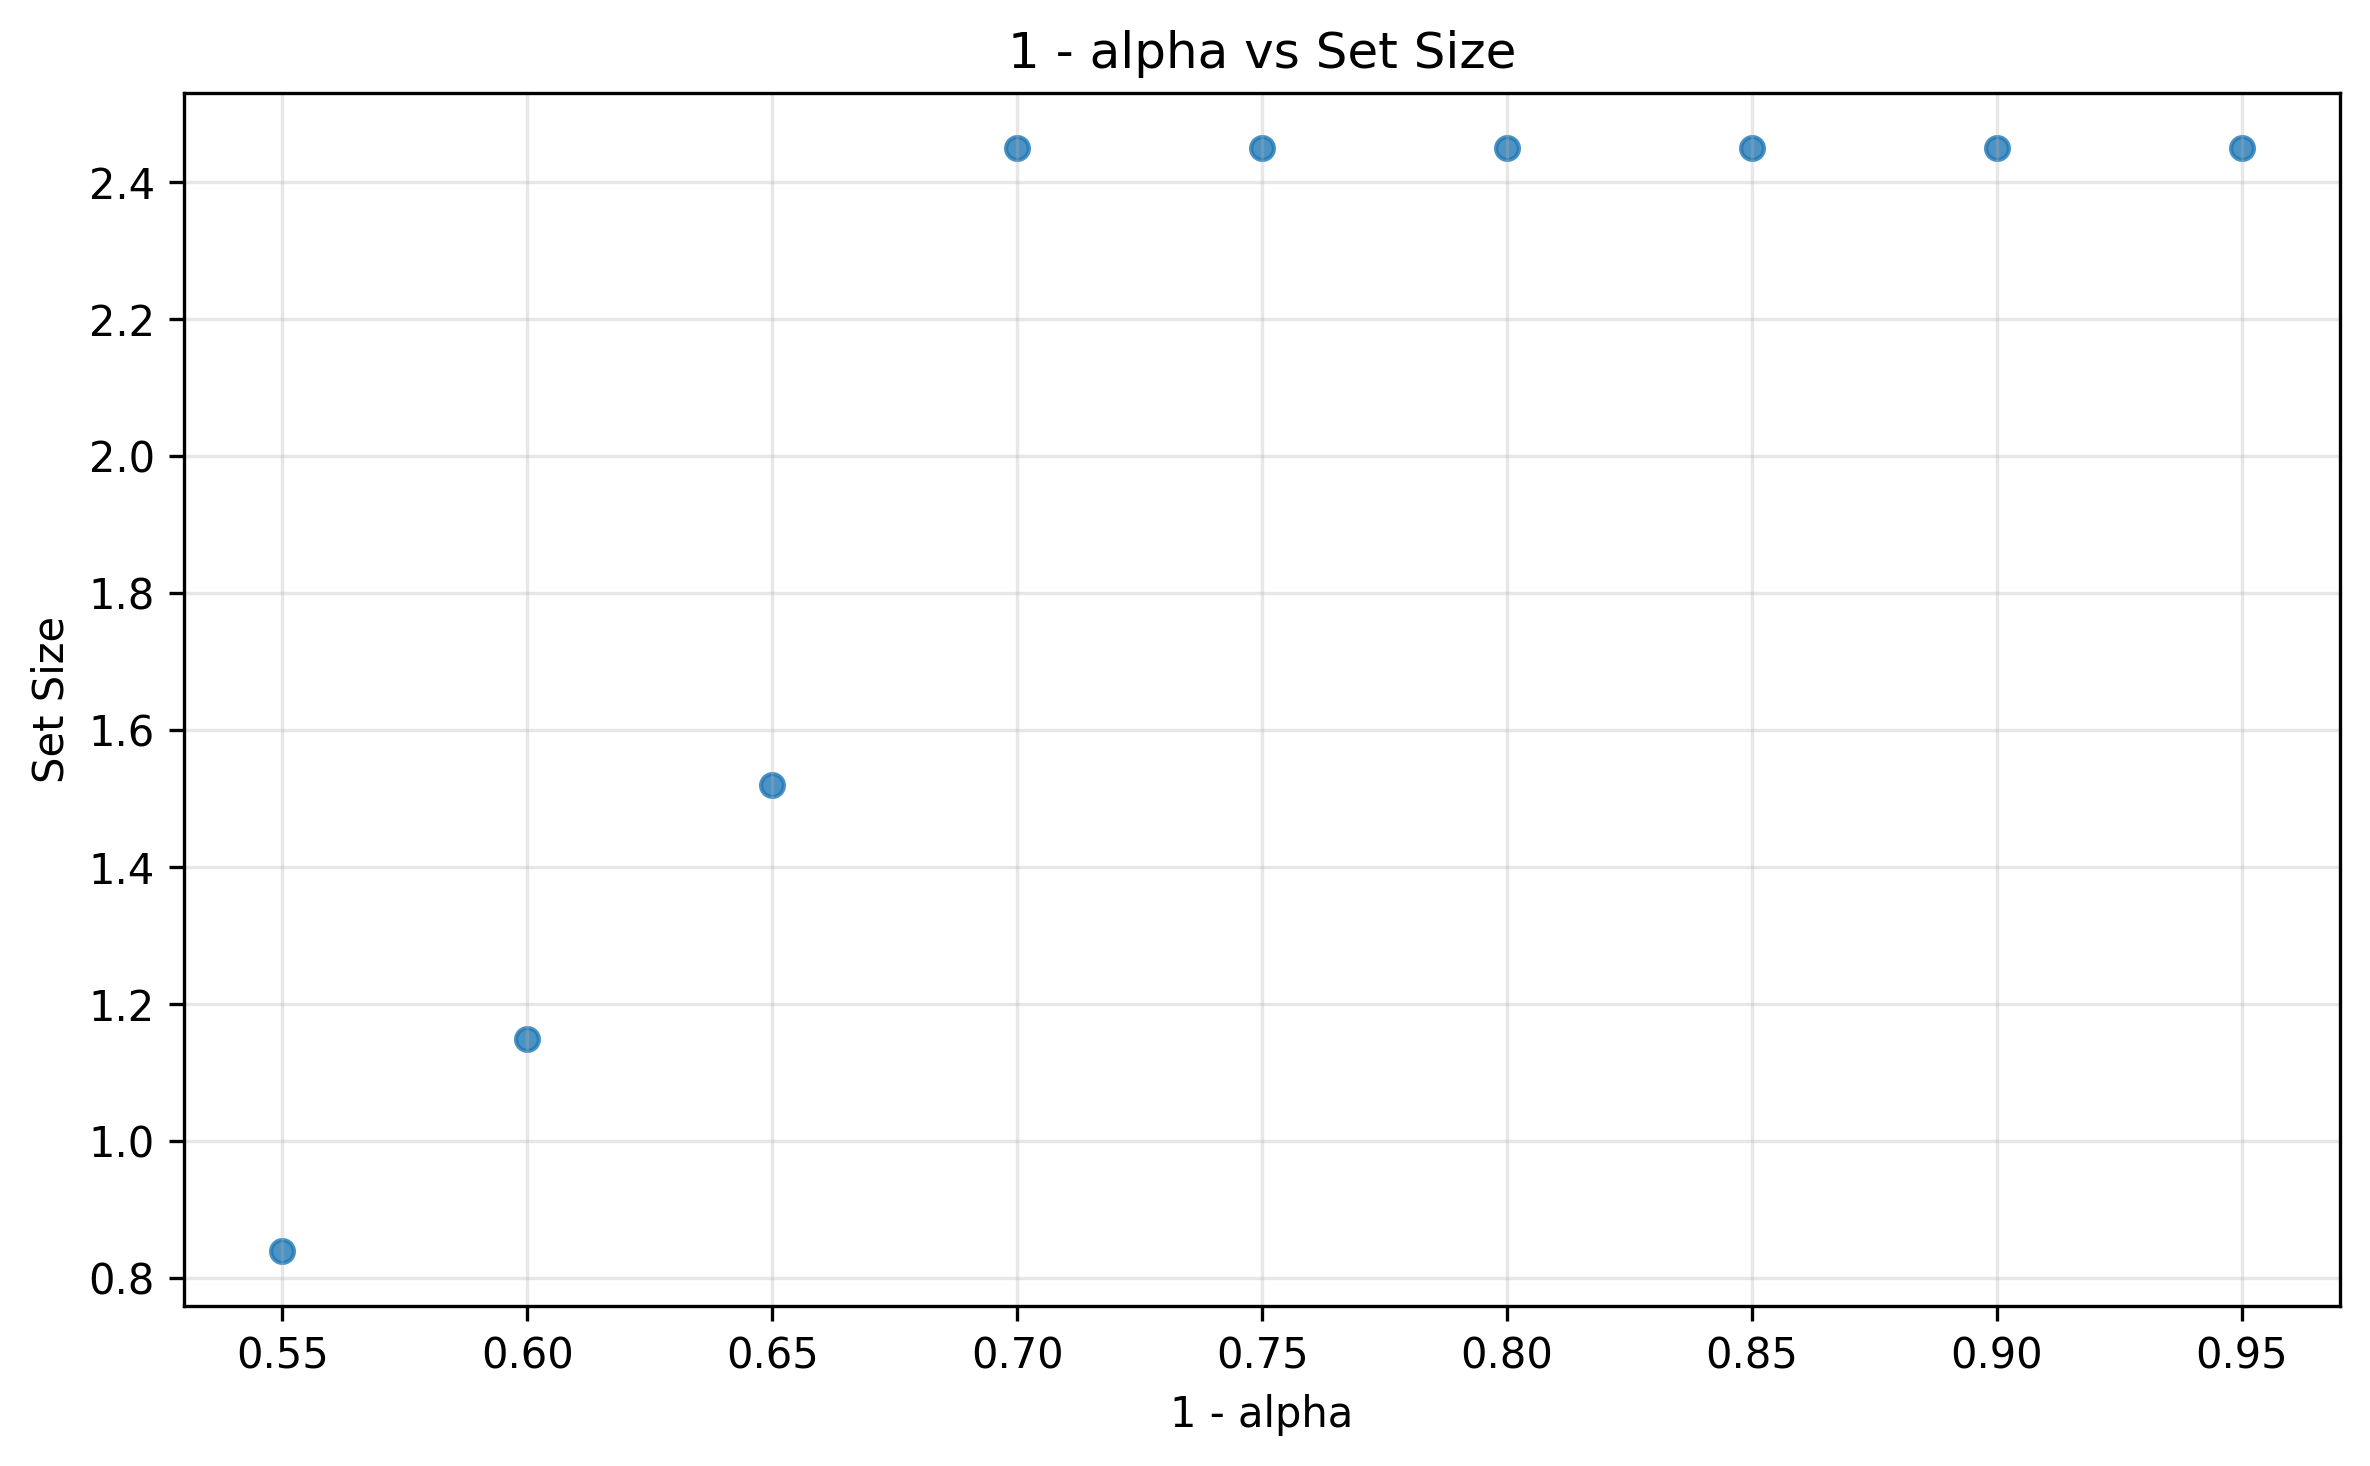
\includegraphics[height=5cm]{cpq/graphs/FreqHighMin1malpha_vs_setsize.png}%
}
\caption{Coverage and set size vs $1 - \alpha$ for the algorithm described above.
  As we can see in the graph, the coverage plateaus, and we cannot guarantee coverage.}
\label{fig:simpleCPQ}
\end{figure}



In order to restore the guarantee of coverage, one option is to introduce an element $EE$ (for \emph{everything else})
into the prediction set. If $EE$ is in the set, then we automatically have coverage.
However, including $EE$ makes our sets much less informative by including an infinite number of options.
Thus, we should try to discourage the presence of $EE$ by making the scores $s(x, EE)$
higher than the scores for actual answers $s(x, y)$.
Our estimate for the probability of $EE$ should be the probability that the answer is \emph{not} any of the answers already seen.
This is the missing probability mass of the clusters: the probability that the answer
is part of everything else not seen in the clusters.
Given this missing mass quantity $\theta(x, t)$, computed from $t$ examples, we define the score
\[ s(x, EE) = 2 - \theta(x, t) , \]
and the score of $y \neq EE$ as
\[ s(x, y) = 1 - \omega(y \mid  x) , \]
where $\omega(y \mid x)$ is the probability of $y$ given the sequence of $t$ samples.
Using the form $2 - \theta$ in the scores $s(x, EE)$ effectively discourages including $EE$ in the prediction set,
since the scores $s(x, EE) \in (1, 2)$ are strictly greater than any scores $s(x, y) \in (0, 1)$.
But how can we measure the missing mass? The \emph{Good--Turing} estimator for the missing mass is
\[ \hat{\theta}(x, t) = \frac{N_1}{t} = \frac{\text{number of clusters that appear exactly $1$ time}}{t} , \]
which is what we use to compute the scores $s(x, EE)$. For the scores of other $y$, we could simply use the frequency-based estimators as earlier, but a more robust strategy is to use a Good--Turing estimator for this as well. If $y$ is seen $r$ times in our $t$ samples, set
\[ \hat{\omega}(y \mid x)  = \frac{r + 1}{t} \frac{N_{r + 1}}{N_r} , \]
where $N_r$ denotes the number of clusters seen exactly $r$ times.
The reason that this is superior to a simple frequency estimate
is that Good--Turing estimators allow for the possibility that the answer is not in the set,
i.e., the estimated probabilities
will not necessarily sum to $1$, so there is some missing mass that is accounted for by the estimators. \medskip

To use this algorithm, one more component is needed. The \emph{query policy} determines the number of times we will sample the model.
Naturally, sampling more is better, but querying the model is expensive and we cannot do it as many times as we please.
The aim is to use a policy that is adaptive to the question
but ensures that the average number of queries is $\le$ the user-set query budget $B$.
The way that we will make our query policy adaptive is to, essentially,
query until the point of diminishing returns.
To quantify this, we again look toward the missing mass. Our policy will be to query until
\[ \theta(x, t + 1) - \theta(x, t) > \beta^* ,\]
where $\beta^*$ is some negative threshold value. In Claim~\ref{querypolicy}, we show that an optimal query policy must have this form.
Effectively, we use the change in $\theta(x, t)$ as a measure of how much information
the query has given us. If the missing mass decreases by only a little, then the query does not add much information,
and we have reached the point of diminishing returns. As far as computing this quantity, we (again) use a Good--Turing estimator. Let
$\Delta(x, t) = \theta(x, t + 1) - \theta(x, t)$. Then our estimator for the change in missing mass is
\[ \hat{\Delta}(x, t) = -\frac{2N_2}{t^2} , \]
where again, $N_2$ is the number of clusters seen exactly twice.
We also have to choose a value of $\beta^*$ that will maintain our query budget $B$.
To do so, we run the query policy over a range of $\beta$ values
and choose the largest value that still has an average number of queries $\le B$.
This full algorithm is known as \emph{CPQ}, introduced in \cite{cpqpaper}.


\begin{figure}[ht]
\centering
\resizebox{\textwidth}{!}{%
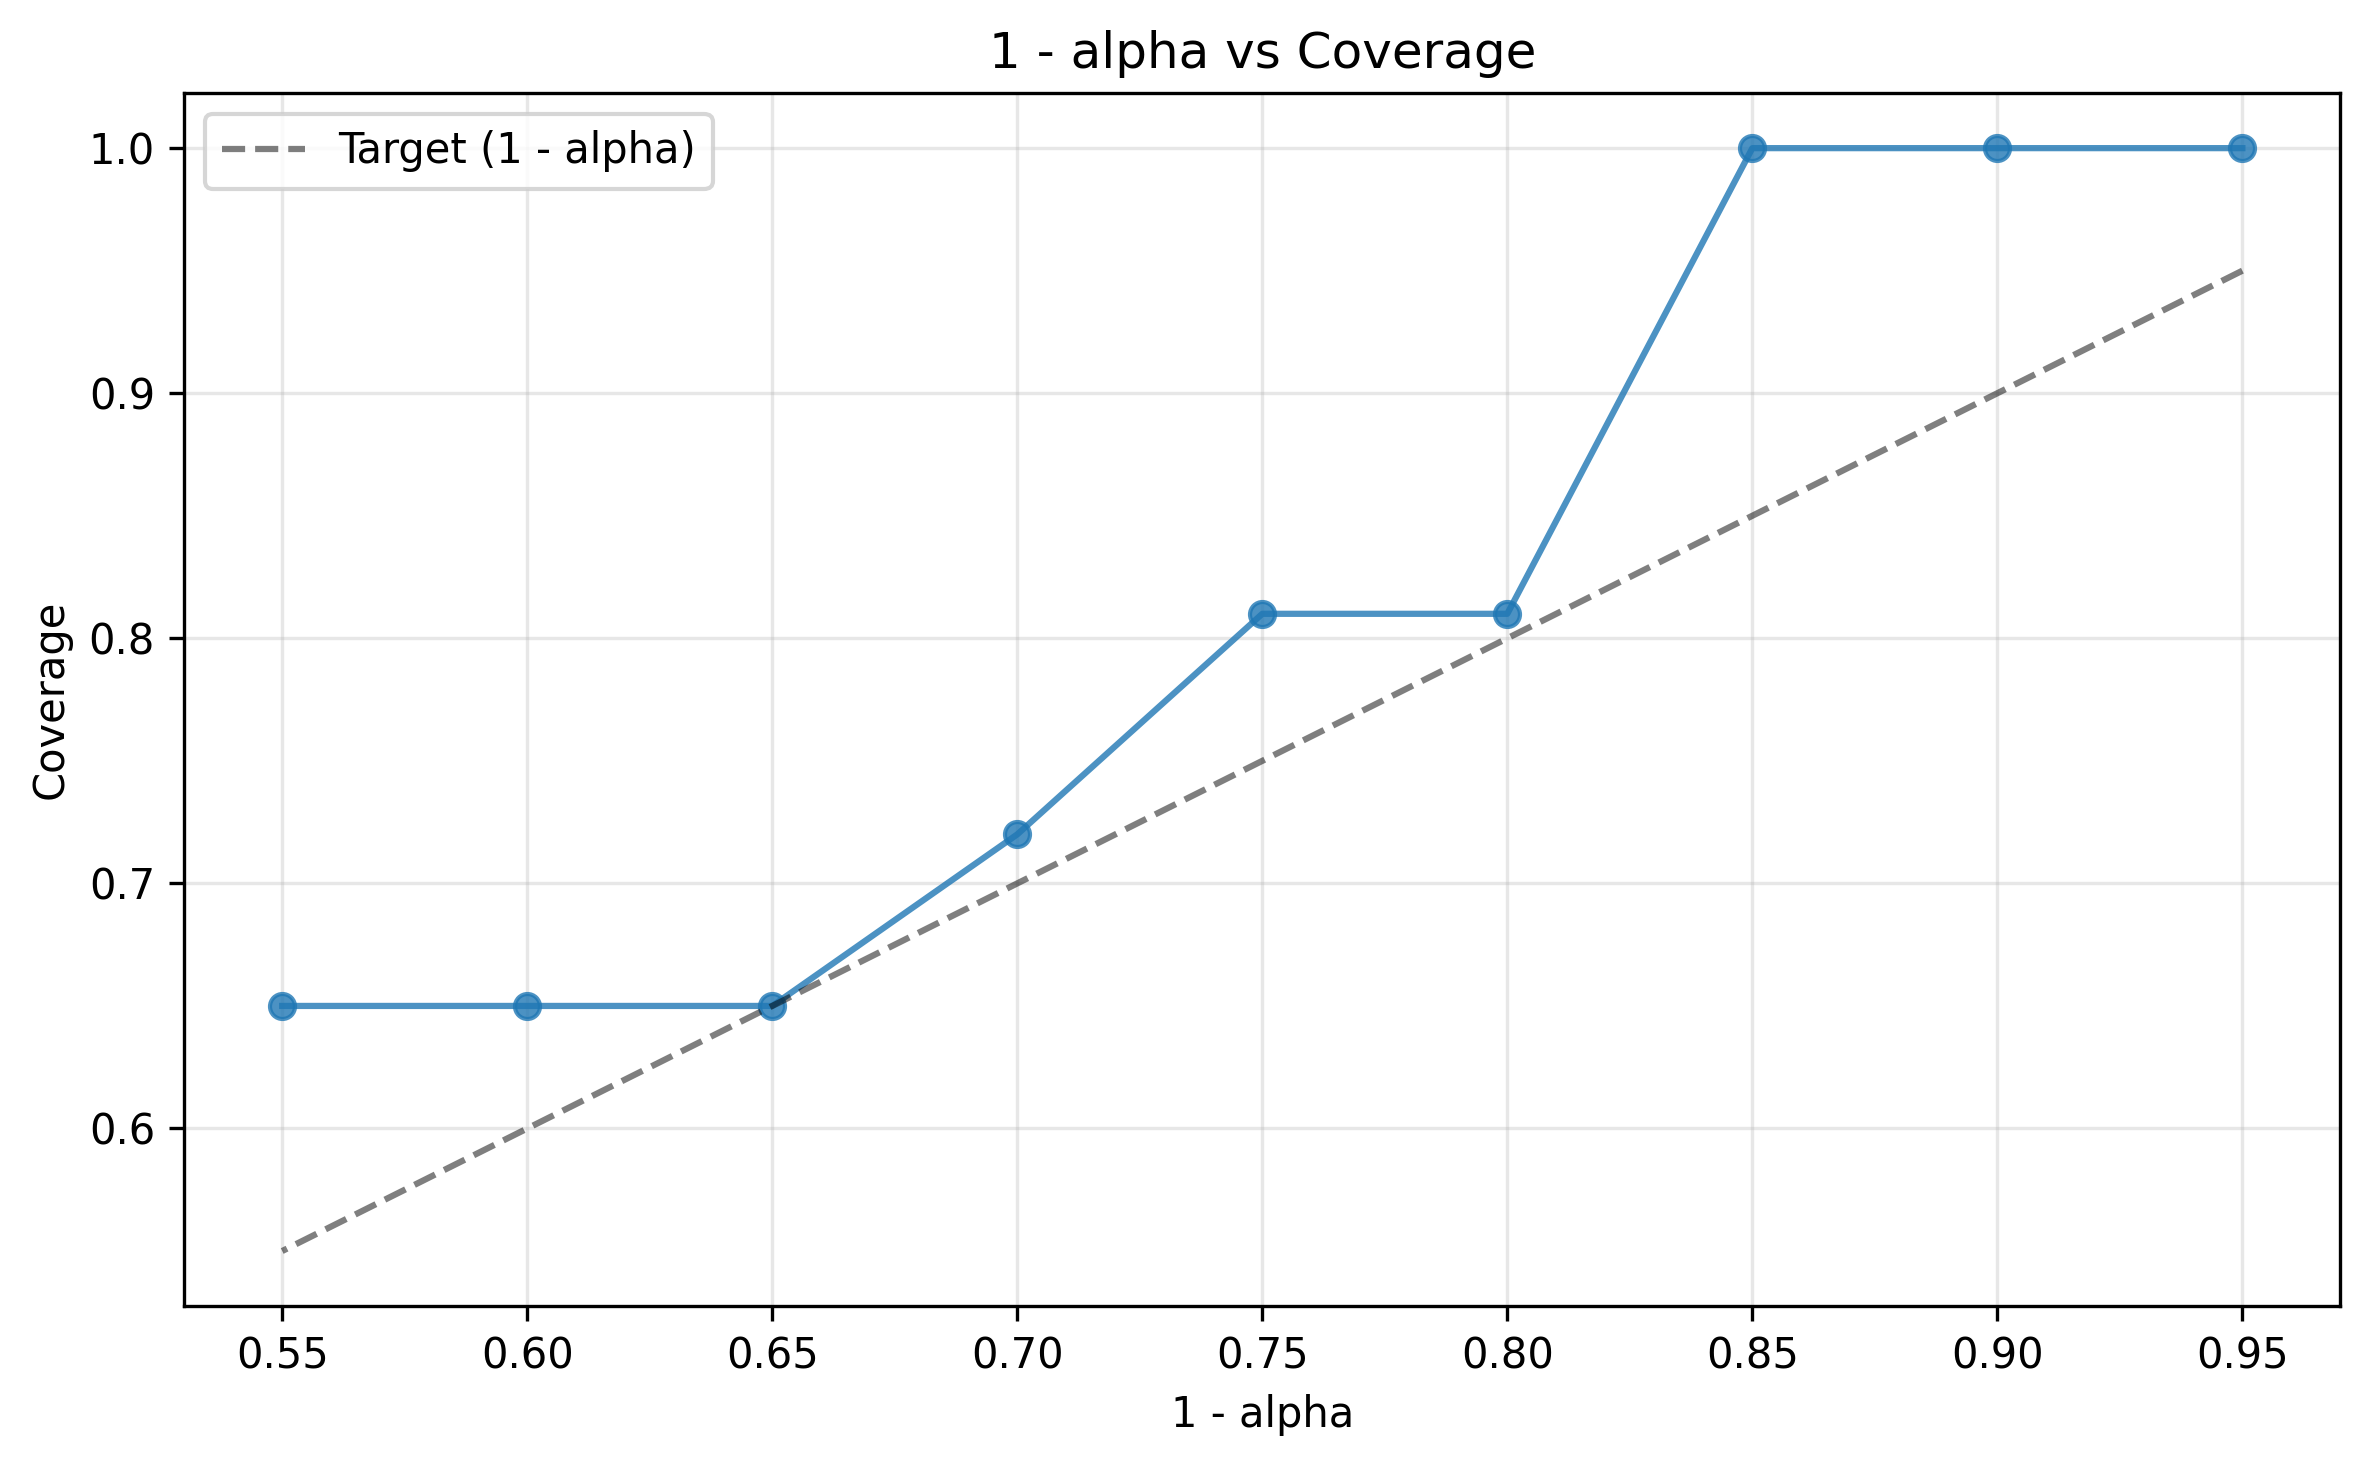
\includegraphics[height=5cm]{cpq/graphs/HighMin1malpha_EE_vs_coverageV1.png}%
\quad
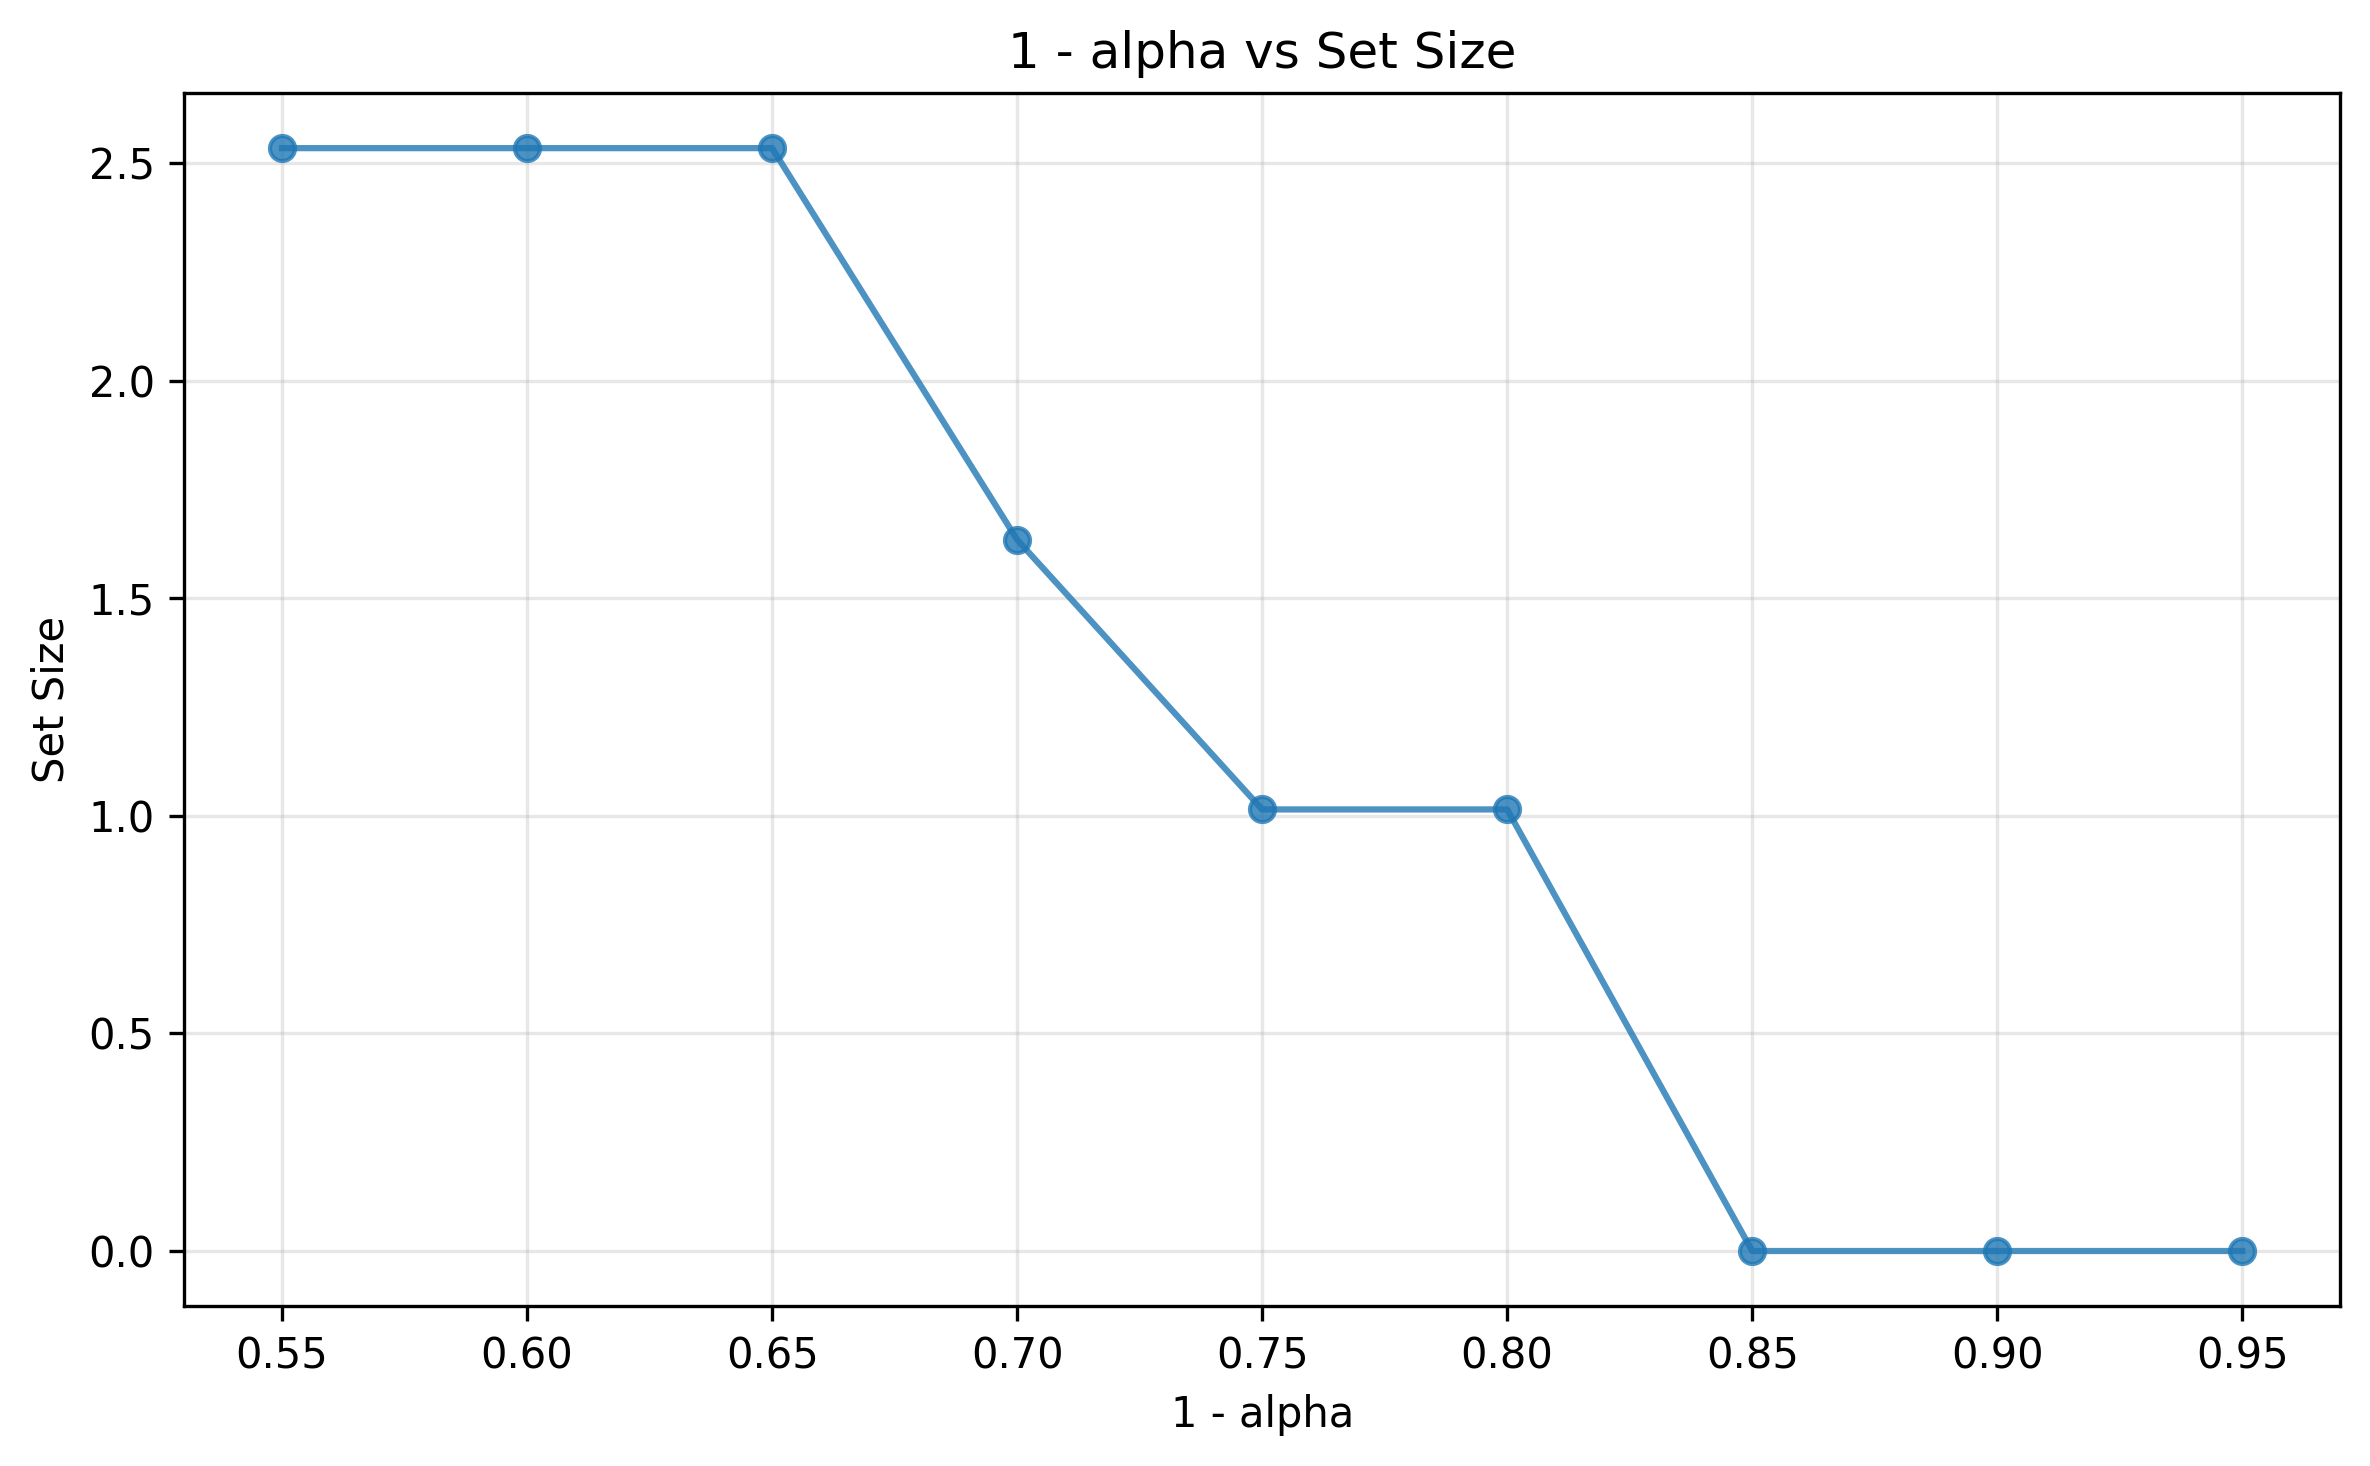
\includegraphics[height=5cm]{cpq/graphs/HighMin1malpha_EE_vs_setsizeV1.png}%
}
\caption{Coverage and set size vs $1-\alpha$ for the CPQ algorithm. The minimum number
of queries was $15$, and Qwen3-8B was the model used both for entailment judging and
for sampling answers on TriviaQA. Here, the sets $\{ EE \}$ were counted with size zero.}
\label{fig:CPQ}
\end{figure}

For this CPQ algorithm, we can also plot the fraction of times $EE$ was included in the prediction set as a metric
for how useful the sets are. The $EE$ fraction vs $1 - \alpha$ plot for our experiment is shown in Figure~\ref{fig:CPQeefrac}.
\begin{figure}[ht]
    \centering
    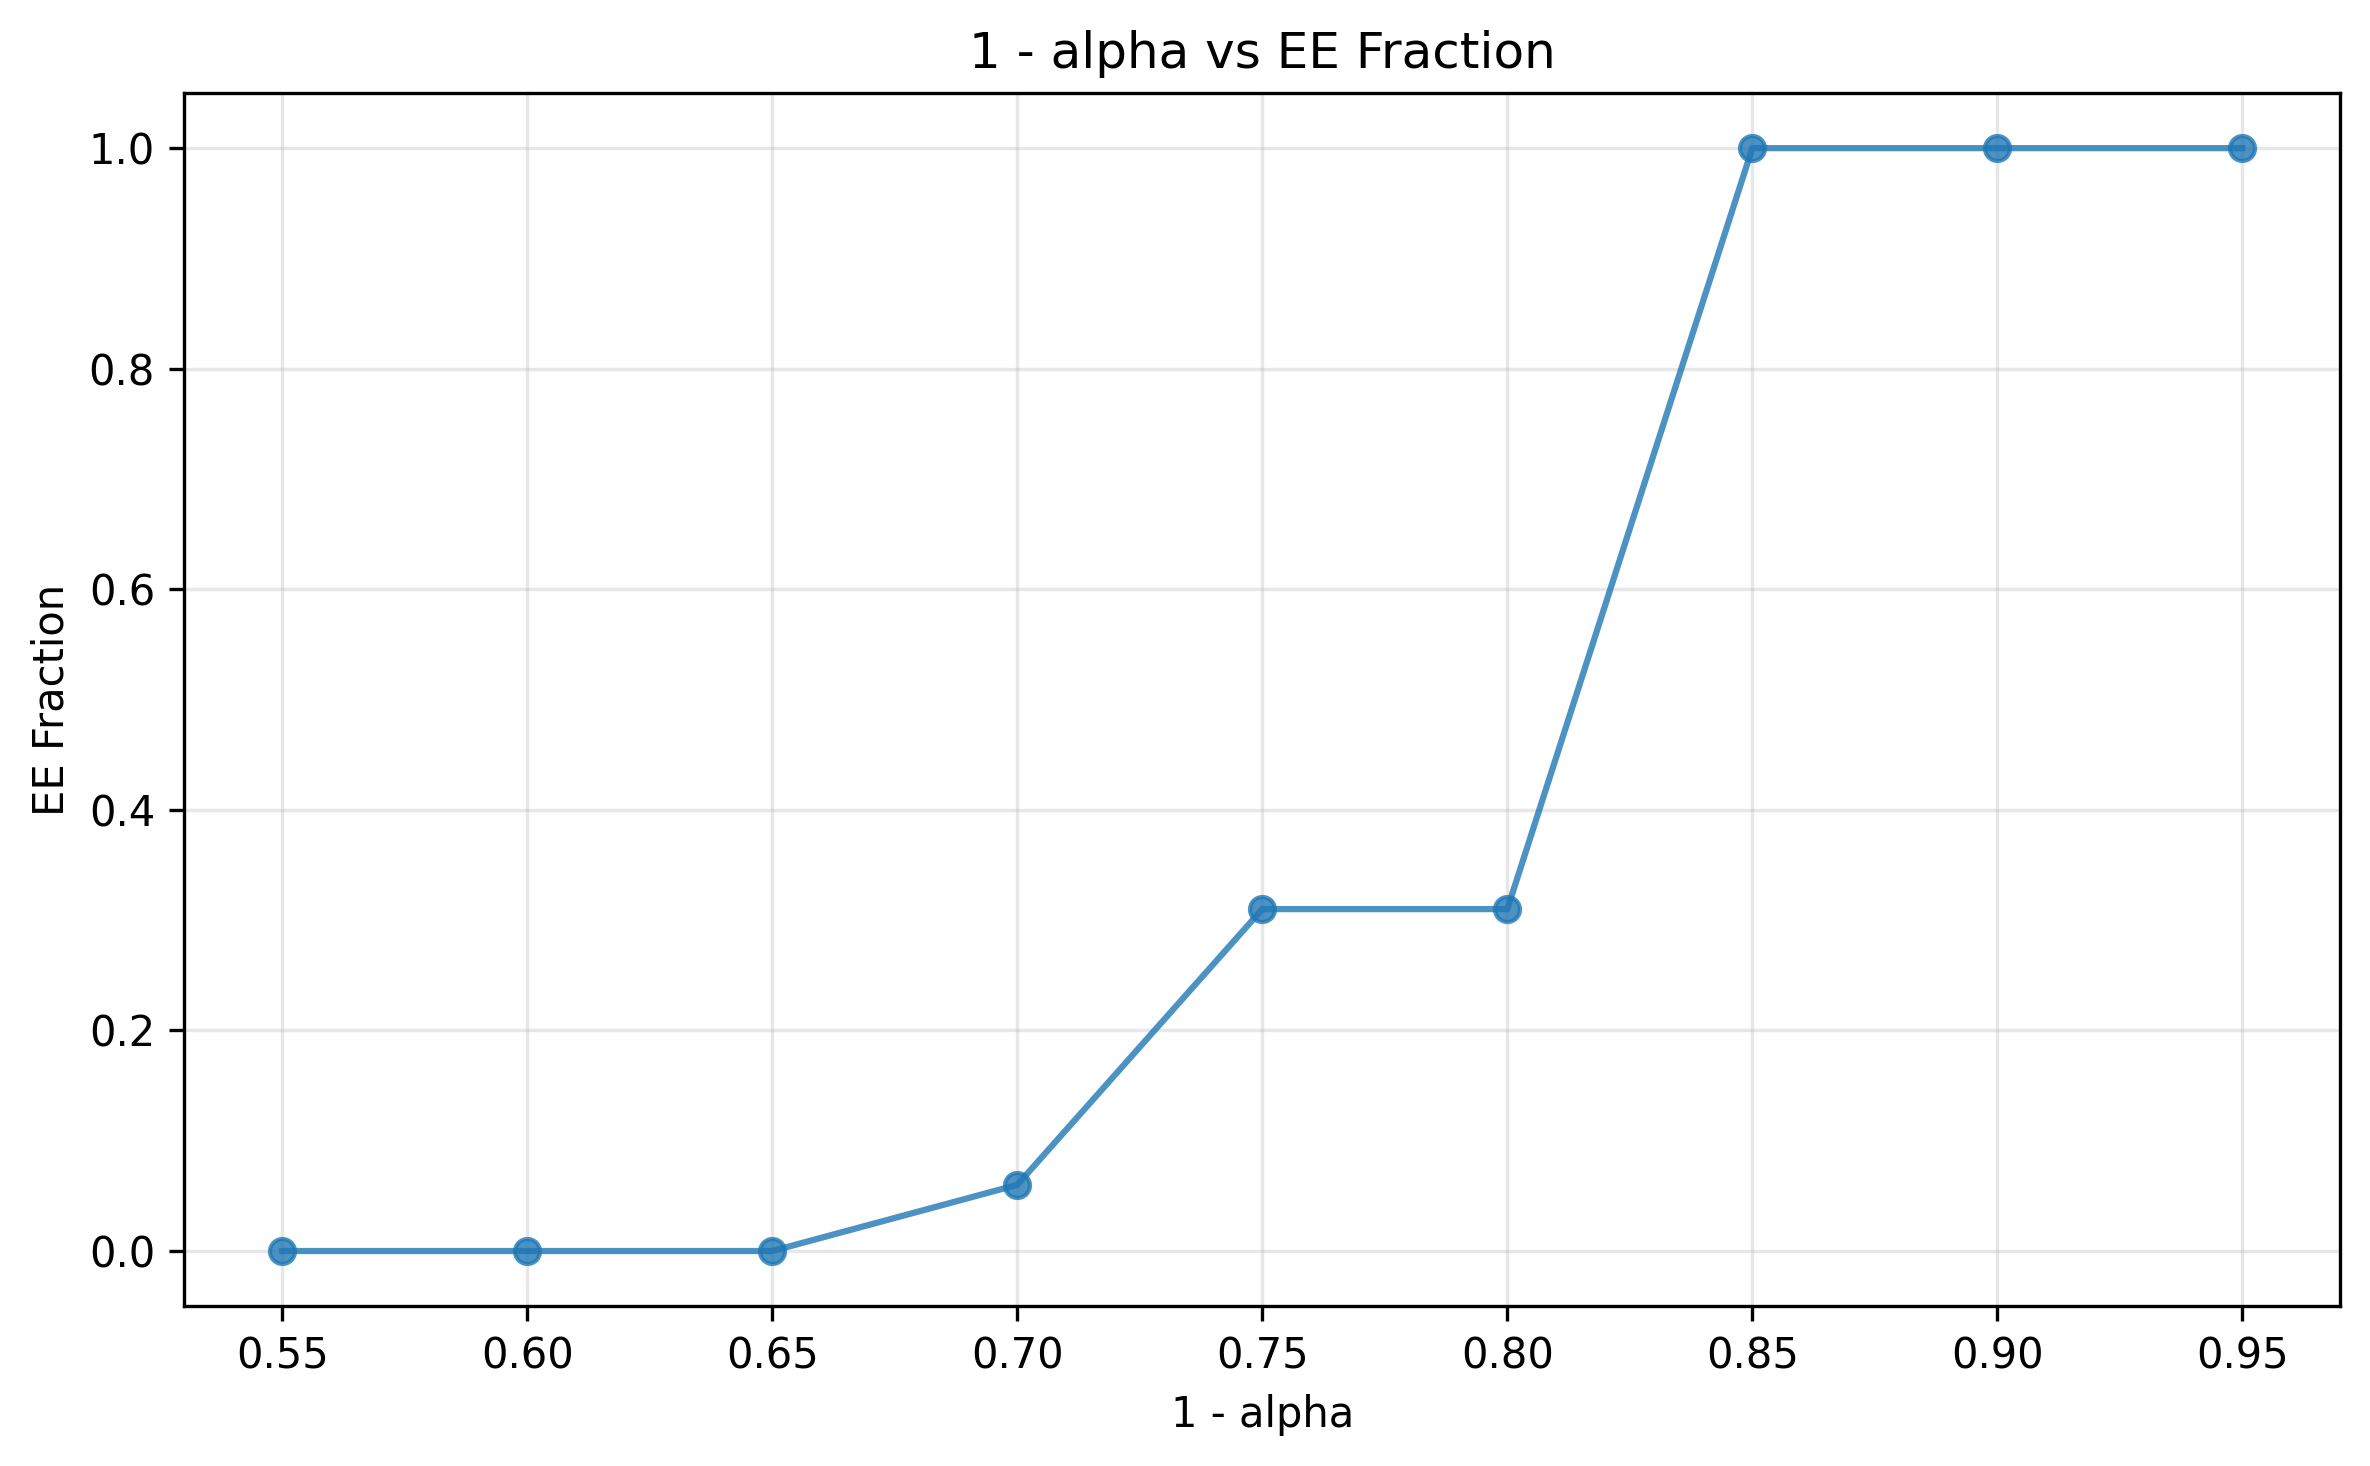
\includegraphics[scale=0.4]{cpq/graphs/HighMin1malpha_EE_vs_eefracV1.png}
    \caption{Fraction of times $EE$ was included vs $1 - \alpha$ for the CPQ algorithm on TriviaQA as above.}
    \label{fig:CPQeefrac}
\end{figure}

As Figure~\ref{fig:CPQ} shows, including $EE$ is able to guarantee coverage when the simple strategy could not.
As the $EE$ fraction increases, the set size decreases, because including $EE$ in the set means we can discard all the other
clusters.
In our experiments, the values of $\hat{q}$ were always $\ge 1$ over the range of $\alpha$ values tested.
This means that any set not containing $EE$ contained every cluster produced by the model,
so the only thing that changed with $\alpha$ was the fraction of the time we returned $\{EE\}$.
This is to be expected when the model has low accuracy: about $45\%$ of the time,
the true answer was not in the generated clusters on the calibration set at all,
and this $0.45$ figure is greater than any of the $\alpha$ values tested, leading to the behavior of $\hat{q} \ge 1$. 
Thus, although we would expect the set size in Figure~\ref{fig:CPQ} to increase before decreasing again, we instead 
only see the decrease. \medskip

\begin{claim}[note=Query Policy, label=querypolicy]
Let $T^* \colon X \to \NN$ be an optimal query policy, in the sense that it minimizes the expected missing mass $E[\theta(x, T(x))]$
over $x \in X$ among all policies $T$ subject to the query budget constraint $E[T(x)] \le B$. Then $T^*$ satisfies
\begin{equation} \Delta(x, T^*(x) - 1) \le \beta^* \le \Delta(x, T^*(x) + 1) \label{idealquery} \end{equation}
for almost every $x \in X$, for some $\beta^*$.
That is, the change in missing mass is $\le \beta^*$ for every query before $T^*(x)$, but greater than $\beta^*$ after query $T^*(x)$.
\end{claim}
\begin{proof}
We assume that we indeed have diminishing returns, that is, $\Delta(x, \cdot)$ is a weakly increasing function.
A proof of this fact is included in \cite{cpqpaper}, as is a more rigorous version of this proof. \medskip

Suppose that $T^*$ is an optimal query policy. We will show that for any value of $\beta$,
either the probability of $\Delta(x, T^*(x) - 1) > \beta$ is $0$, or the probability of $\Delta(x, T^*(x) + 1) < \beta$ is $0$.
These inequalities are simply the negations of those in \eqref{idealquery}.
The result follows from this, since we can select $\beta_1$ to be the smallest value for which $P(\Delta(x, T^*(x) - 1) > \beta) = 0$
and $\beta_2$ to be the largest value for which $P(\Delta(x, T^*(x) + 1) < \beta) = 0$.
If $\beta_1 > \beta_2$, there would be a value in between them for which both of the probabilities being considered are nonzero,
which is a contradiction. Thus, $\beta_2 \ge \beta_1$, and we can choose $\beta^*$ to satisfy $\beta_2 \ge \beta^* \ge \beta_1$. \medskip

Let $R$ be a subset of $X$ such that $\Delta(x, T^*(x) - 1) > \beta$ for all $x \in R$,
and let $S$ be a subset of $X$ with $\Delta(x, T^*(x) + 1) < \beta$ for all $x \in S$, such that $p(R) = p(S)$.
Both $R$ and $S$ can be chosen nonempty because we have assumed both events happen with positive probability,
and $X$ is assumed to have a continuous distribution. If $x \in R$, we have over-queried with $T^*$, and we can do one fewer query and still get a $\Delta$ value greater than $\beta$.
Similarly, if $x \in S$, we have under-queried, and can query one more time and still get a $\Delta$ value greater than $\beta$. As such, define
\[ T'(x) = \begin{cases*}
        T^*(x) - 1 & \text{if $x \in R$,} \\
        T^*(x) + 1 & \text{if $x \in S$,} \\
        T^*(x) & \text{otherwise.}
    \end{cases*}
\]
We show that $T'$ is strictly better than $T^*$. Firstly, $E[T'(x)] = E[T^*(x)]$
because we have chosen $p(R) = p(S)$; this means that we adjust up with the same probability as we adjust down.
In particular, $T'$ still obeys the query budget constraint. Moreover, if $x \in R$ is an over-query, we can see that
\[ \theta(x, T^*(x)) - \theta(x, T'(x)) = \theta(x, T^*(x)) - \theta(x, T^*(x) - 1) = \Delta(x, T^*(x) - 1) > \beta . \]
Analogously, if $x \in S$ is an under-query, we see
\[ \theta(x, T^*(x)) - \theta(x, T'(x)) = -\Delta(x, T^*(x)) \ge -\Delta(x, T^*(x) + 1) > -\beta , \]
which follows from the diminishing returns property. But now,
\begin{align*}
&E[\theta(x, T^*(x))] - E[\theta(x, T'(x))] \\
&= E[\theta(x, T^*(x)) - \theta(x, T'(x))] \\
&= p(R)E_{x \in R}[\theta(x, T^*(x)) - \theta(x, T'(x))] + p(S)E_{x \in S}[\theta(x, T^*(x)) - \theta(x, T'(x))] \\
&> p(R)\beta + p(S)(-\beta) \\
&= 0 .
\end{align*}
That is, $T'$ has lower expected missing mass than $T^*$, so it is better, contradicting the assumption that $T^*$ is optimal.
Thus, we have shown that for any $\beta$, either the probability of $\Delta(x, T^*(x) - 1) > \beta$ is $0$, or the probability of $\Delta(x, T^*(x) + 1) < \beta$ is $0$.
\end{proof}

\printbibliography
\end{document}